\chapter{Discussion}
\label{chap:discussion}

Intro discussion ? Poor performance?

\section{Overfitting}
\label{sec:overfitting}

A recurring problem for the models trained for this thesis is the number of predictions that are identical to a label found in the training set.
When this occurs, it shows that a model is not able to achieve the task of predicting a de novo molecular representation from \ac{MS/MS}, but only repeats the data is has been trained with.
There are a few contributing factors to this overfitting problem with the setup used in this thesis.

\subsection{Duplicate training labels}
As mentioned in the paper from MassSpecGym \cite{bushuiev2024massspecgym}, the dataset is a collection of the most qualitative annotated open-source mass spectrometry datasets.
Even though a lot of filtering was performed after thorough quality control, the amount of duplicate molecules is significant.
Figure \ref{fig:duplicate_smiles} shows the amount of SMILES that have multiple occurrences in the training set. Notice the logarithmic y-axis for readability.
Even though 84\% of unique molecules have 10 occurrences or less, some molecules are noticeably more present in the training set, with one molecule being present 477 times in the training set.
This imbalance does not necessarily reflect the real-world imbalance of molecules as it is caused by the use of imbalanced datasets.
This causes the models to be trained with a bias towards these more frequent occurring molecules in the training set.
This imbalance is also present in the validation (and test) set, where the most frequently occurring molecule accounts for 2.7\% (out of the almost 20.000 entries) of the validation data.
Because of this imbalance, the models will be evaluated with a bias towards these more abundant molecules.
\begin{figure}[h]
    \centering
    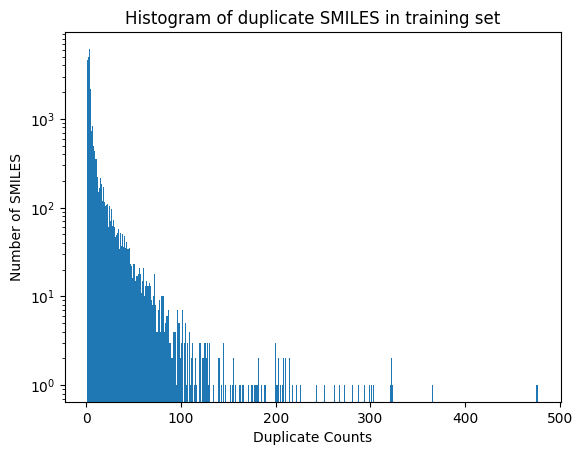
\includegraphics[width=0.6\textwidth]{figures/discussion/duplicate_smiles_training_set.png}
    \caption{distribution of duplicate SMILES in MassSpecGym's training set with a logarithmic scale}.
    \label{fig:duplicate_smiles}
\end{figure}

\subsection{Exposure bias}

During training, a teacher forcing approach is used, where only the ground truth tokens are used to generate the next token iteratively.
At inference time, when the model is sampled, the model does not get this help and has to rely on its own previous (incorrect) predictions.
This is often referred to as exposure bias \cite{schmidt2019generalization}.
The previously discussed imbalance of the training set only makes this bias worse, by training on these frequently occurring token combinations.
This severely hinders the generalization of the model.
An example of this exposure bias can be clearly seen in the results from the hyperparameter gridsearch (figure \ref{fig:gridsearch_vs_paper}), where a model with a lower validation loss performed after sampling.
The loss has this teacher forced advantage, while the metrics calculated on the sampled predictions do not.
Because all models trained in this thesis are optimized for validation loss, it can be questioned if they have been overfit on these teacher forced training molecules.

\subsection{Evaluation metrics}
The two metrics used to evaluate similarity of a molecular prediction, Tanimoto similarity and \ac{MCES} distance, are somewhat flawed.
As explained in section \ref{sec:tan_sim}, the Tanimoto similarity uses molecular fingerprints that are unable to store all structural information.
When the predicted structure is converted to a molecular fingerprint, some structural information is lost.
The prediction will thus not be evaluated completely.
The \ac{MCES} distance on the other hand does evaluate the whole molecular structure, but can in some cases behave sub-optimal.
Looking at the formula in section \ref{sec:mces_dist}, when the evaluation molecules have few edges in their molecular graphs, a model could instead of finding the \acf{MCES}, just minimize the edges in its prediction.
In an extreme case, where the model only predicts nothing (e.g. empty SMILES), the MCES distance will be equal to the number of edges of the ground-truth molecule.
While during training the model does not have access to the MCES distance and will thus probability not reach this extreme case, it does question if some \ac{MCES} distances have been sugarcoated by this flaw.

Another problem with both metrics is that they are unable to distinguish between de novo and training molecules.
This can cause problems when the models are not powerful enough to outperform overfitted models.
A model that, instead of predicting de novo molecules, would just rank the training molecules and return the most similar ones (similar to frequently used database lookup methods), could appear relatively good at predicting de novo molecules when only the \ac{MCES} distance and Tanimoto similarity are considered.
Only the number of novel molecules accurately shows if a model can generate de novo molecules.
Hence, to compare models, and decide which is better at predicting de novo molecules form \ac{MS/MS}, multiple metrics have to be considered.


\section{Results Experiments}

Most of the results from the experiments in this thesis show no clear improvements over the methods used by the de novo models from MassSpecGym.
However, many conclusions can still be drawn from these results.
In hindsight, some experiments could still be improved upon by taking the results and discussion points from \ref{sec:overfitting} into account.
The following sections discuss the results and possible improvements for each experiment.

\subsection{Samplers benchmark}

The main conclusion from the samplers benchmark is that different samplers can perform better with different evaluation settings.
The deterministic samplers performed best with top-1 evaluation, showing their capability to predict valid molecules.
The probabilistic samplers, on the other hand, predicted more varying, sometimes invalid, molecules, which allowed them to outperform the deterministic samplers with a top-10 evaluation setting.

When predicting molecular structures from \ac{MS/MS}, randomness is not a desired property as there is only one correct molecular structure.
Even though multiple SMILES can represent the same molecular structure, overall we only want the correct atoms and bonds to be predicted.
A possible explanation for this phenomenon is that, on average, a bit of randomness could somewhat overcome the exposure bias from the overfitted model.

In later experiments, it shows that the SMILES model used for this experiment was severely overfit on the training SMILES.
This experiment should in an ideal case also have to be repeated for a model that is able to predict more de novo molecules (e.g. SELFIES model).

\subsection{\ac{BPE} as pretraining}

Using \ac{BPE} increases the number of valid predictions at the cost of novel predictions. 
This conclusion is again confirmed by the molecular representations experiment in figure \ref{fig:representations}.
The main advantage is that by grouping multiple tokens as one, \ac{BPE} decreases the number of tokens the model has to predict.
When the model has less tokens to predict, it will make less mistakes, leading to more valid molecules.
In contrast, it will favour grouped tokens seen in the training data, and by having less tokens to predict, it will more often lead to predictions from the training set.
When using \ac{BPE}, the parameters of the algorithm should be tuned such that a balance between performance and minimal overfitting could be found.

While the results show that computing the \ac{BPE} on the 118M dataset did not improve the model's performance compared to the 4M dataset, even though it has almost 30 times more SMILES,
the quality of this dataset is considerably worse.
As explained in the MassSpecGym paper, the 118M dataset consists of all the available data from PubChem. 
No quality control was conducted for this dataset, which allows for an unrealistic distribution of chemical classes in the dataset.
An overrepresentation of one chemical class could severely influence the patterns found by the \ac{BPE} algorithm.
In contrast, the 4M dataset does have a controlled representation of multiple chemical classes.
This shows that quality is preferred over quantity.

\subsection{Augmentation}

- again only one model used which experienced overfitting
Only BPE encoded SMILES models, overfitting might influence results

\subsubsection*{SMILES augmentation}
- SMILES from molecular graph is deterministic, evaluation is done on only these deterministic outputs, by randomizing the SMILES with synonyms it confuses the model and will perform worse on the evaluated SMILES.
- model not powerfull enough
- BPE does not help because augmented patterns use more tokens
- less augmentation
- could maybe be usefull to replace the duplicate SMILES

\subsubsection*{Spectral augmentation}

Confirms DreaMS results
Could be used to fix molecule imbalance, where only the least occurring molecules in the training set are augmented


\subsection{Molecular representations benchmark}

Models not optimized for hyperparameters
samplers chosen based of SMILES results

3 headed inchi could be improved by supplying the output of the previous decoder to the next, to ensure they know what molecule it is trying to predict

explain DeepSMILES BPE flaw?

SELFIES can benefit from BPE because some tokens have different meaning in context of rings and groups, without the model overfitting

\section{Future for de novo structure prediction}

All models still severely struggle to predict only a few molecular structures completely from the validation set.
- autoregressive models not suited for molecular structure generation by exposure bias
- string based representations not suited, reference graph based paper
